% !TEX program = xelatex
\documentclass[11pt,a4paper]{article}

\usepackage{fontspec}
\usepackage[a4paper,left=2.7cm,right=6.3cm,top=2.5cm,bottom=2.6cm,
            marginparwidth=4.5cm,marginparsep=0.7cm,footskip=1.3cm]{geometry}
\usepackage{xcolor}
\usepackage{booktabs}
\usepackage{tabularx}
\usepackage{array}
\usepackage{tcolorbox}
\usepackage{tikz}
\usepackage{titlesec}
\usepackage{enumitem}
\usepackage{microtype}
\usepackage{ragged2e}
\usepackage{fancyhdr}
\usepackage[hidelinks]{hyperref}
\usetikzlibrary{positioning,arrows.meta,calc,fit,backgrounds,shapes.geometric}
\tcbuselibrary{skins,breakable}

% ---------------------------------------------------------------- palette ---
\definecolor{ink}{HTML}{16191A}
\definecolor{bodyc}{HTML}{2C3230}
\definecolor{muted}{HTML}{5C6360}
\definecolor{faint}{HTML}{8A918D}
\definecolor{rulec}{HTML}{D3D7D2}
\definecolor{sunk}{HTML}{EFF1ED}
\definecolor{accent}{HTML}{2E5D57}
\definecolor{accentsoft}{HTML}{DFE9E6}
\definecolor{warn}{HTML}{8A5E18}
\definecolor{warnsoft}{HTML}{F3E9D8}
\definecolor{fatal}{HTML}{8E2F28}
\definecolor{fatalsoft}{HTML}{F5E2DF}
\definecolor{termbg}{HTML}{1A1F1E}
\definecolor{termink}{HTML}{D9DED9}
\definecolor{termdim}{HTML}{7E8A85}
\definecolor{termac}{HTML}{7FBFB1}

% ------------------------------------------------------------------ fonts ---
\setmainfont{Charter}[Numbers=OldStyle, Ligatures=TeX]
\setsansfont{Avenir Next}[Ligatures=TeX]
\setmonofont{Menlo}[Scale=0.82]
\newfontfamily\displayfont{Avenir Next}[Ligatures=TeX]
\newfontfamily\labelfont{Avenir Next}[Letters=Uppercase, LetterSpace=14.0, Ligatures=TeX]
\newfontfamily\tabfont{Avenir Next}[Ligatures=TeX, Numbers=Lining]

\color{bodyc}
\linespread{1.14}
\setlength{\parindent}{0pt}
\setlength{\parskip}{0.62em}
\setlength{\emergencystretch}{2em}

% --------------------------------------------------------------- sections ---
\titleformat{\section}[block]
  {\displayfont\bfseries\fontsize{15.5}{18}\selectfont\color{ink}}
  {\color{accent}\fontsize{13}{13}\selectfont\thesection\hspace{0.7em}}{0pt}{}
\titlespacing*{\section}{0pt}{1.95em plus .3em minus .2em}{0.7em}

\titleformat{\subsection}[block]
  {\displayfont\bfseries\fontsize{11}{13}\selectfont\color{ink}}{}{0pt}{}
\titlespacing*{\subsection}{0pt}{1.5em plus .2em minus .1em}{0.35em}

% ---------------------------------------------------------------- helpers ---
\newcommand{\lab}[1]{{\labelfont\fontsize{7.4}{9}\selectfont\color{accent}#1}}
\newcommand{\mlab}[1]{{\labelfont\fontsize{7.4}{9}\selectfont\color{faint}#1}}
\newcommand{\note}[1]{\marginpar{\RaggedRight\sffamily\fontsize{7.8}{10.4}\selectfont\color{muted}#1}}
\newcommand{\notel}[2]{\marginpar{\RaggedRight\sffamily\fontsize{7.8}{10.4}\selectfont%
  \lab{#1}\\[0.35em]\color{muted}#2}}

\newcommand{\hairline}{\vspace{0.35em}{\color{rulec}\hrule height 0.4pt}\vspace{0.55em}}

% terminal block
\newtcolorbox{term}{breakable, colback=termbg, colframe=termbg, boxrule=0pt,
  arc=1.5pt, left=10pt, right=8pt, top=8pt, bottom=8pt,
  fontupper=\ttfamily\fontsize{7.8}{11.2}\selectfont\color{termink}}
\newcommand{\tc}[1]{\textcolor{termdim}{#1}}
\newcommand{\tk}[1]{\textcolor{termac}{#1}}
\newcommand{\tw}[1]{\textcolor[HTML]{D2A055}{#1}}
\newcommand{\tf}[1]{\textcolor[HTML]{DC7A6F}{#1}}

% pull quote
\newtcolorbox{pull}[1][]{breakable, colback=sunk, colframe=sunk, boxrule=0pt,
  leftrule=2pt, colbacktitle=sunk, borderline west={2pt}{0pt}{accent},
  arc=0pt, left=11pt, right=11pt, top=9pt, bottom=9pt, #1}

% table helpers
\newcolumntype{L}[1]{>{\RaggedRight\arraybackslash}p{#1}}
\newcolumntype{Y}{>{\RaggedRight\arraybackslash}X}
\newcolumntype{C}{>{\centering\arraybackslash}X}
\newcolumntype{K}[1]{>{\RaggedRight\leavevmode\color{ink}\arraybackslash}p{#1}}
\newcommand{\thd}[1]{\leavevmode{\labelfont\fontsize{7}{8.5}\selectfont\color{faint}#1}}
\newcommand{\tb}[1]{{\color{ink}#1}}
\renewcommand{\arraystretch}{1.48}
\newcommand{\tabstyle}{\tabfont\fontsize{8.4}{10.6}\selectfont\color{bodyc}\setlength{\parskip}{0pt}\linespread{1.0}\selectfont}

% wide float that eats into the margin column
\newcommand{\wide}[1]{\noindent\makebox[\textwidth][l]{%
  \begin{minipage}{\dimexpr\textwidth+\marginparsep+\marginparwidth\relax}#1\end{minipage}}}

% --------------------------------------------------------------- headfoot ---
\pagestyle{fancy}\fancyhf{}
\renewcommand{\headrulewidth}{0pt}
\fancyfoot[R]{\sffamily\fontsize{8}{8}\selectfont\color{faint}\thepage}
\fancyfoot[L]{\labelfont\fontsize{6.8}{8}\selectfont\color{faint}NULLIUS IN VERBA}

\begin{document}

% ============================================================== TITLE ======
\thispagestyle{empty}
\vspace*{0.6cm}
\noindent{\labelfont\fontsize{8}{10}\selectfont\color{accent}A HARNESS FOR RESEARCH WORK}

\vspace{0.5em}
\noindent{\displayfont\bfseries\fontsize{46}{46}\selectfont\color{ink}Nullius}

\vspace{0.9em}
\noindent\begin{minipage}{\textwidth}
{\color{rulec}\hrule height 0.5pt}
\vspace{0.9em}
{\fontsize{21}{25}\selectfont\itshape\color{ink}nullius in verba}\\[0.5em]
{\sffamily\fontsize{10.5}{14}\selectfont\color{ink}“Take nobody's word for it.”}\\[0.7em]
{\sffamily\fontsize{8.6}{12.6}\selectfont\color{muted}The Royal Society's motto since 1660, and the
oldest continuous statement of the discipline this harness enforces. Then the unreliable narrator
was authority. Now it is a fluent model, an author's own abstract, and you. Same job.}
\vspace{0.9em}
{\color{rulec}\hrule height 0.5pt}
\end{minipage}

\vspace{1.4em}
\noindent\begin{minipage}{\textwidth}
{\fontsize{12.5}{17}\selectfont\color{ink}This document is the argument, not the manual. It says
what an AI assistant does wrong in research work by default, why writing better instructions does
not fix it, and what a harness has to constrain instead.}
\end{minipage}

\vspace{1.1em}
\noindent{\sffamily\fontsize{8.4}{12.4}\selectfont\color{muted}%
The short version: research has no compiler, so the design problem is finding what plays that
part. Seven things do. Everything else in the tool is built on top of them, and nothing that
cannot fail is allowed to block.}

\vspace{2.2em}

% ============================================================== 1 ==========
\section{The motto is the specification}
\notel{why it is not decoration}{Every mechanism in the design is an instance of one sentence.
That is a rare property in a name, and it doubles as a consistency check: a mechanism that is not
a conjugation of the motto probably does not belong.}

Names are usually labels. This one is a specification. \emph{Nullius in verba} was adopted by the
Royal Society in 1660 as a refusal to settle questions by citing authority, and every constraint
in this harness turns out to be that sentence pointed at a different narrator.

\vspace{0.3em}
\wide{%
\par\vspace{0.45em}{\tabstyle\begin{tabularx}{\linewidth}{K{4.6cm} Y}
\toprule
\thd{DO NOT TAKE} & \thd{THE MECHANISM} \\
\midrule
the author's word & an \texttt{authors-claim} may never be written as a bare assertion \\
the abstract's word & warrant is capped by how deeply you actually read \\
the field's word & \texttt{established} is computed from author-set overlap, never declared \\
the repeated word & folklore is a citation trail that never reaches data \\
your own word & your unpublished data is held to a published paper's bar \\
the reviewer's word & a \texttt{defensible} finding closes with one sentence, permanently \\
\bottomrule
\end{tabularx}}\par\vspace{0.5em}}

The last row is the one people are surprised by, and it is the reason this is a harness rather
than a critic. Taking nobody's word for it cuts both ways: an unexamined objection is no better
than an unexamined claim, and a tool that can always find one more thing wrong has stopped
providing evidence and started providing pressure.

% ============================================================== 2 ==========
\section{What goes wrong by default}
\notel{observed, not imagined}{These are failures seen in real sessions. The clearest one: a
research proposal that grew from 12 pages to 24 across three runs, where the fourth still
returned a list of what was missing.}

None of this is the model being lazy. Each is a place where nothing in the loop \emph{could} fail,
so the default filled the gap.

\subsection{It skims the literature and does not know it}
Four papers, one query, one afternoon, written up as \emph{“a review of the literature on X”}.
The prose form hides it perfectly: one query and forty look identical on the page. Worse, the
search runs in \emph{your} vocabulary rather than the field's, so an entire literature can sit
one synonym away and never appear.

\subsection{It trusts a paper the way the paper describes itself}
An abstract is a marketing document. What a study \emph{shows} is in its tables, and the gap
between the two is where most of the interesting reading happens. By default that gap is
collapsed: the claimed contribution and the evidenced contribution arrive as one sentence.

\subsection{It cannot tell settled from proposed}
This is the expensive one. \emph{“Attention improves long-range modelling”} and \emph{“method Y
improves long-range modelling”} come out in the same declarative mood at the same confidence.
One carries a decade of independent replication; the other carries one paper and one benchmark.
Build three chapters on the second believing it was the first, and you find out late.

\subsection{Its critique has no floor}
Asked what is missing, it answers. Asked again, it answers again. \emph{More} reads as \emph{more
rigorous}, so a finished draft becomes an infinite project, and a page limit that was never
declared cannot object. The 12-to-24 story above is not a pathology; it is the predictable
output of an unbounded question asked four times.

\begin{pull}
\lab{THE ASYMMETRY THAT MAKES THIS HARD}\\[0.5em]
Suppress \emph{“what is missing”} and a genuinely absent control section goes unmentioned. Leave
it unbounded and the draft doubles and is still called incomplete. A single rule cannot serve
both, which is why the two have to stop being one axis.
\end{pull}

% ============================================================== 3 ==========
\section{Why more instructions do not fix it}
\notel{measured, not asserted}{The predecessor of this design replaced a 43{,}494-word instruction
collection, plus 9{,}572 words loaded on every turn, with six hooks and one ledger. Every rule in
the prose was a request; none could fail. That is why a rule had to be repeated three to five
times before it took effect.}

The instinct is to write the rule more firmly. \emph{Search thoroughly. Verify before claiming.
Do not overstate.} These are not wrong. They constrain the wrong thing.

A rule that describes \emph{how} to work has no truth value. Nothing can check it, so it competes
for attention with everything else in the context and loses whenever the task gets interesting. A
constraint on \emph{what must hold} has a truth value: it can be observed, it costs nothing until
it fires, and it leaves the approach entirely alone.

\vspace{0.3em}
\wide{%
\par\vspace{0.45em}{\tabstyle\begin{tabularx}{\linewidth}{K{6.2cm} Y}
\toprule
\thd{PROCESS CONSTRAINT · UNENFORCEABLE} & \thd{OUTCOME CONSTRAINT · ENFORCEABLE} \\
\midrule
“survey the literature first” & a survey unit cannot close with unscreened $>0$ \\
“don't over-trust the paper” & a claim may not exceed its source's read depth \\
“distinguish settled from new” & \texttt{established} requires disjoint author sets \\
“cite accurately” & an unresolved identifier cannot reach the draft \\
“say what done means” & an acceptance question that is open right now \\
“don't pad it” & over budget, an addition must name what it costs \\
“know when to stop” & zero material findings is a verdict, not a shorter list \\
\bottomrule
\end{tabularx}}\par\vspace{0.5em}}

Each row on the right is a state the session can be observed to be in. That is the whole
difference, and it is why this is a set of gates rather than a longer prompt.

% ============================================================== 4 ==========
\section{Research has no compiler}
\notel{the honest floor}{It is a short list, and it is enough. Shallow is invisible in prose and
undeniable in a row of numbers.}

Software gets this for free. \emph{It builds}, \emph{the suite is green}, \emph{the check went red
to green} are facts, observed rather than reported, and facts can block. Research has no
equivalent, so the entire design question is: which questions here are \emph{equally} objective?

Seven are, and every one is a lookup or a count. None asks the model to judge quality.

\vspace{0.3em}
\wide{%
\par\vspace{0.45em}{\tabstyle\begin{tabularx}{\linewidth}{K{7.4cm} Y}
\toprule
\thd{QUESTION} & \thd{THE CHECK} \\
\midrule
Does this reference exist? & the identifier resolves, or it does not \\
Was it retracted or corrected? & retraction metadata on the record \\
Does the paper say this? & the quote is verbatim in the cached text, or it is not \\
Are these two sources independent? & author and institution sets: disjoint, or not \\
Does this claim's trail reach data? & walk the references back and see where it lands \\
Did you search the field's words? & distinct query vocabularies, with hit counts \\
Is a required section absent? & the venue's own list, walked \\
\bottomrule
\end{tabularx}}\par\vspace{0.5em}}

Two of those are the cheapest real epistemics available and nobody builds them. \textbf{Source
independence is set arithmetic on author lists.} \textbf{Folklore is a citation trail that never
lands on evidence.} Both fall out of metadata already fetched to render a bibliography.

\begin{term}
\tc{\$ nullius coverage}\\[0.35em]
found\ \ \ \ \ \ \ \tw{231}\ \ \ \ screened \tf{0}\ \ \ \ \ included\ \ \ \tw{4}\\
vocabularies \tf{1}\ \ \ \ \tc{of 3 required --- try the field's terms, not yours}\\
groups\ \ \ \ \ \ \tf{1}\ \ \ \ \tc{4 works, 2 shared authors, not independent}\\
years\ \ \ \ \ \ \ 2024--2026\ \ \tc{most-cited ancestor of the seed set unread}
\end{term}

\emph{“I reviewed the literature”} survives any amount of scrutiny. That block does not.

% ============================================================== 5 ==========
\section{Warrant, capped by read depth}
\notel{the strongest single rule}{You cannot talk your way past it, because the note recorded how
far you read \emph{before} the claim existed.}

Every claim carries a warrant class saying what settles it. The class that matters most is the one
nobody tracks: \texttt{authors-claim}, meaning \emph{the authors assert this}, recorded separately
from what their tables show.

Then the cap. A paper note records how far you actually got --- abstract, skim, method, replicated
--- and \textbf{a claim may not exceed the read depth of its source.}

\vspace{0.3em}
\wide{%
\par\vspace{0.45em}{\tabstyle\begin{tabularx}{\linewidth}{K{2.6cm} C C C C}
\toprule
\thd{READ DEPTH} & \thd{“THEY REPORT X”} & \thd{“X HOLDS”} & \thd{“THEIR METHOD SHOWS WHY”} & \thd{“THIS GENERALISES”} \\
\midrule
abstract   & \textcolor{accent}{ok} & \textcolor{fatal}{refused} & \textcolor{fatal}{refused} & \textcolor{fatal}{refused} \\
skim       & \textcolor{accent}{ok} & \textcolor{accent}{ok} & \textcolor{fatal}{refused} & \textcolor{fatal}{refused} \\
method     & \textcolor{accent}{ok} & \textcolor{accent}{ok} & \textcolor{accent}{ok} & \textcolor{fatal}{refused} \\
replicated & \textcolor{accent}{ok} & \textcolor{accent}{ok} & \textcolor{accent}{ok} & \textcolor{accent}{ok} \\
\bottomrule
\end{tabularx}}\par\vspace{0.5em}}

This works where an instruction does not because the difference is \emph{textual}. \emph{“They
report a 12\% gain”} and \emph{“the method gives a 12\% gain”} are different strings, and the
ledger holds the class. A script can decide it. \emph{“Be appropriately skeptical”} cannot be
decided by anything.

% ============================================================== 6 ==========
\section{Settled versus proposed}
\notel{orthogonal axes}{Warrant asks \emph{how do you know this}. Status asks \emph{how settled is this in the field}.}

Epistemic status is a second axis, and it is the one that costs years when it is missing. The
failure is not citing something false; it is citing something \emph{true but unsettled} as though
it were settled.

\vspace{0.3em}
\wide{%
\par\vspace{0.45em}{\tabstyle\begin{tabularx}{\linewidth}{K{2.5cm} L{5.2cm} Y}
\toprule
\thd{STATUS} & \thd{WHAT EARNS IT} & \thd{HOW IT MAY APPEAR IN PROSE} \\
\midrule
textbook & graduate texts treat it as background & bare assertion \\
established & \emph{independent} replication, disjoint author sets & bare assertion, review cited \\
contested & serious work on both sides, both logged & must name both sides \\
emerging & one or two groups, recent & “early evidence suggests”, groups counted \\
single-result & one paper, one setting & attributed and situated, never bare \\
folklore & repeated; the trail never reaches data & marked unsourced, or dropped \\
\bottomrule
\end{tabularx}}\par\vspace{0.5em}}

Two things stop status from being self-declared. It is \textbf{capped by source independence} ---
the exact parallel to the read-depth cap, and computable from author identifiers the record
already carries. And its rendering is greppable, so the discipline lives in a difference a script
can see rather than in an adjective the model is asked to feel.

Pointed the other way, the same axis is what stops your open question from being closed on your
behalf: a live disagreement rendered as \texttt{contested} keeps a door open that a confident
summary would have quietly shut.

% ============================================================== 7 ==========
\section{Missing, or merely more}
\notel{the hardest arbitration}{And the one the 12-to-24 story needed --- note that it is not a judgement call.}

Back to the asymmetry. The resolution is that \emph{“something is missing”} is three different
claims wearing one word, and they differ in whether they can point at something enumerable.

\vspace{0.3em}
\wide{%
\par\vspace{0.45em}{\tabstyle\begin{tabularx}{\linewidth}{K{2.8cm} L{5.2cm} Y}
\toprule
\thd{KIND} & \thd{GROUNDED IN} & \thd{WHY IT TERMINATES} \\
\midrule
structural & the venue's list of required sections & the checklist is finite \\
evidential & the claim ledger & the claims are enumerable \\
coherence & two locations in the artifact & the pairs are finite \\
\textcolor{fatal}{enhancement} & \textcolor{fatal}{nothing} & \textcolor{fatal}{it never does} \\
\bottomrule
\end{tabularx}}\par\vspace{0.5em}}

So: \textbf{a finding must cite a required-section id, a claim id with an empty warrant, or two
conflicting locations. A finding that cites none of the three is enhancement, and inadmissible.}
No severity intuition required --- a finding either has a referent or it does not.

The same rule keeps the tool honest in the other direction. The completeness sweep is
\textbf{walked, not sampled}: every required section gets present, thin or absent, every run.
\emph{“It never told me the timeline was missing”} cannot happen, because the checklist is
enumerated rather than intuited. And “required” comes from a real document --- the grant call, the
author guidelines, the venue's checklist, the field's reporting standard --- so the tool cannot
invent a requirement it can't cite.

\subsection{The budget is a price, not a ceiling}

Now the two axes compose. A gap is real or it is not; the artifact is inside its format or over
it. Four situations, one honest answer each.

\vspace{0.6em}
\wide{%
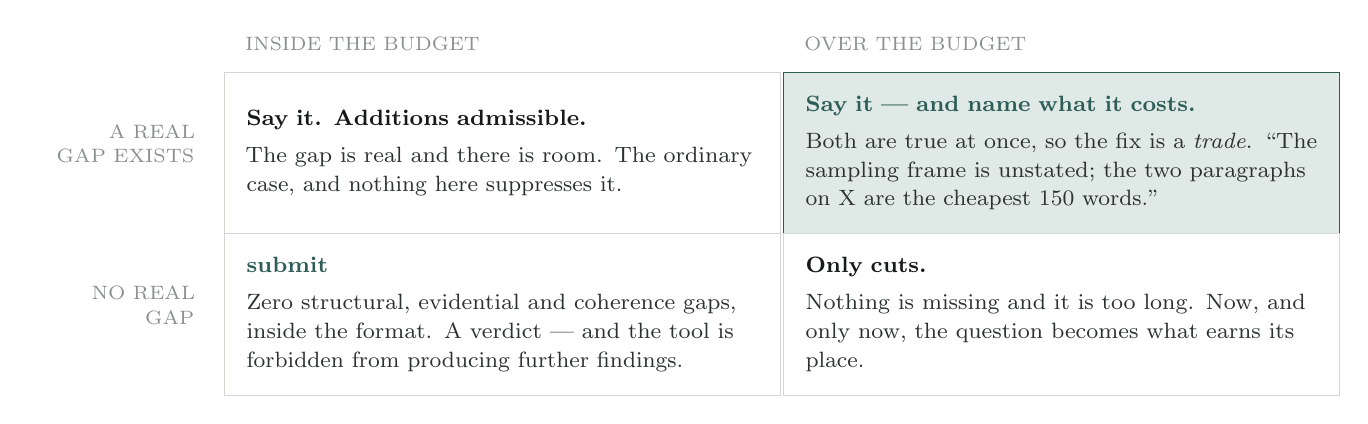
\begin{tikzpicture}[
  font=\tabfont\fontsize{8.2}{10.4}\selectfont,
  cell/.style={draw=rulec, line width=0.4pt, rectangle, minimum width=7.0cm,
               minimum height=2.05cm, align=left, text width=6.5cm, inner sep=8pt,
               anchor=north west, text=bodyc},
  hd/.style={font=\labelfont\fontsize{7}{7}\selectfont, text=faint, anchor=south west},
  rh/.style={font=\labelfont\fontsize{7}{9}\selectfont, text=faint, anchor=north east,
             align=right, text width=2.0cm},
]
\node[hd] at (0.15,0.15) {INSIDE THE BUDGET};
\node[hd] at (7.25,0.15) {OVER THE BUDGET};

\node[rh] at (-0.25,-0.55) {A REAL\\GAP EXISTS};
\node[cell] at (0,0) {{\bfseries\color{ink}Say it. Additions admissible.}\\[3pt]
  The gap is real and there is room. The ordinary case, and nothing here suppresses it.};
\node[cell, fill=accentsoft, draw=accent] at (7.1,0) {{\bfseries\color{accent}Say it --- and name what it costs.}\\[3pt]
  Both are true at once, so the fix is a \emph{trade}. “The sampling frame is unstated; the two
  paragraphs on X are the cheapest 150 words.”};

\node[rh] at (-0.25,-2.6) {NO REAL\\GAP};
\node[cell] at (0,-2.05) {{\bfseries\color{accent}submit}\\[3pt]
  Zero structural, evidential and coherence gaps, inside the format. A verdict --- and the tool is
  forbidden from producing further findings.};
\node[cell] at (7.1,-2.05) {{\bfseries\color{ink}Only cuts.}\\[3pt]
  Nothing is missing and it is too long. Now, and only now, the question becomes what earns its
  place.};
\end{tikzpicture}}

\vspace{0.9em}
The upper-right cell is the one that fourth run needed and did not have. And the funding
requirement is a severity filter the tool \textbf{cannot fake}: nobody trades two working
paragraphs for a nice-to-have, so soft findings collapse under their own price without anyone
having to judge them soft.

\begin{pull}
\lab{THE REFRAME}\\[0.5em]
The budget does not forbid additions. It \textbf{prices} them --- and a priced list has to be
ranked, while a free list can only be enumerated. An unbounded set of improvements becomes a
ranked set of trades, and a ranked set has a top and therefore a bottom.\\[0.6em]
The switch from \emph{“what is missing”} to \emph{“what earns its place”} is then nobody's
judgement call. It happens on its own, the moment the last real gap closes.
\end{pull}

% ============================================================== 8 ==========
\section{What blocks, and what is merely reported}
\notel{why the split matters more here}{Almost everything worth saying about research is a
calibrated judgement. If those blocked, the harness would become the thing it exists to prevent.}

A fact and a chosen number are different claims, and conflating them is how a good gate turns into
a nuisance. Facts block. Thresholds that were picked rather than measured are reported, and marked
as chosen.

\vspace{0.7em}
\wide{%
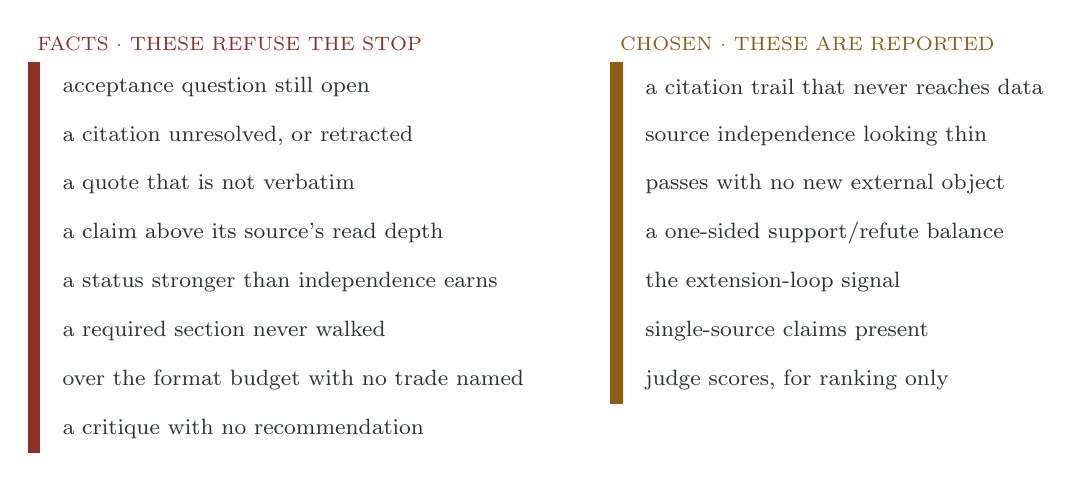
\begin{tikzpicture}[
  font=\tabfont\fontsize{8}{10}\selectfont,
  row/.style={anchor=west, text=bodyc},
  bar/.style={rectangle, minimum height=0.62cm, minimum width=0.16cm, inner sep=0pt},
]
\node[font=\labelfont\fontsize{7}{7}\selectfont, text=fatal, anchor=west] at (0,0.55) {FACTS · THESE REFUSE THE STOP};
\foreach \i/\txt in {
  0/{acceptance question still open},
  1/{a citation unresolved, or retracted},
  2/{a quote that is not verbatim},
  3/{a claim above its source's read depth},
  4/{a status stronger than independence earns},
  5/{a required section never walked},
  6/{over the format budget with no trade named},
  7/{a critique with no recommendation}}{
  \node[bar, fill=fatal] at (0.08,-\i*0.62) {};
  \node[row] at (0.32,-\i*0.62) {\txt};
}
\node[font=\labelfont\fontsize{7}{7}\selectfont, text=warn, anchor=west] at (7.4,0.55) {CHOSEN · THESE ARE REPORTED};
\foreach \i/\txt in {
  0/{a citation trail that never reaches data},
  1/{source independence looking thin},
  2/{passes with no new external object},
  3/{a one-sided support/refute balance},
  4/{the extension-loop signal},
  5/{single-source claims present},
  6/{judge scores, for ranking only}}{
  \node[bar, fill=warn] at (7.48,-\i*0.62) {};
  \node[row] at (7.72,-\i*0.62) {\txt};
}
\end{tikzpicture}}

\vspace{0.5em}
The left column needs no calibration to be right. The right column would need a hundred or two
labelled examples and an agreement measure before it could honestly refuse anything, and that work
has not been done --- so it does not refuse. Saying which is which is not a caveat. It is the
difference between a gate you trust and one you learn to route around.

% ============================================================== 9 ==========
\section{Making it yours}
\notel{why it can be open}{The plugin holds no opinion about your field. Everything
field-specific is a file you write, which is also what makes it publishable.}

A harness that hard-coded one field's norms would be useless in every other field and quietly
wrong in its own. So the tool ships knowing nothing, and the norms are configuration:

\begin{itemize}[leftmargin=1.1em, itemsep=0.25em, topsep=0.4em]
\item \texttt{field.md} --- your subfield's norms. What a normal sample size is here, what a
  standard baseline is, which claims need what kind of evidence. This is what makes a critique
  \emph{calibrated} rather than idealised.
\item \texttt{venues/<venue>.md} --- required sections, page limit, what reviewers there actually
  ask for. Bootstrapped once from the real call or author guidelines. A structural finding must
  cite a line in this file, so the tool cannot invent a requirement.
\item \texttt{program.md} --- what you are actually working on, so a thread that does not trace
  to it can be flagged as the distraction it is.
\item \texttt{threads/}, \texttt{papers/}, \texttt{claims.md}, \texttt{falsified.md} --- the
  durable record. This is the half that survives a dead context window, and a dead semester.
\end{itemize}

\begin{pull}
\lab{THE ONE FILE PEOPLE UNDERESTIMATE}\\[0.5em]
\texttt{falsified.md} holds the ideas you killed and why. It costs a minute to write and it is
the only thing standing between you and re-proposing, in June, the idea you buried in March.
\end{pull}

% ============================================================== 10 =========
\section{What this is not}
\notel{stated plainly}{A research tool that overstates itself would be an unusually poor joke.}

\begin{itemize}[leftmargin=1.1em, itemsep=0.3em, topsep=0.4em]
\item \textbf{Not a literature database.} It queries real indexes --- OpenAlex, Crossref,
  Semantic Scholar, arXiv, Unpaywall, Europe PMC --- through their official APIs. Coverage is
  theirs, and it is uneven by field. The tool's contribution is refusing to let you \emph{not}
  look, not pretending the index is complete.
\item \textbf{Not a substitute for reading.} The read-depth cap exists precisely because the tool
  cannot read for you. It can only refuse to let an abstract masquerade as a method section.
\item \textbf{Not a calibrated judge.} The severity classes rank; they do not measure. Where a
  number was chosen rather than measured, the tool says so and does not block on it.
\item \textbf{Not a way around a paywall.} Official APIs and legally open full text only.
\item \textbf{Not an author.} It has no opinion about what you should study, and the parts that
  look like opinions are your own \texttt{field.md} read back to you.
\end{itemize}

% ============================================================== 11 =========
\section{Where this is}
\notel{honest status}{Design settled, build starting. This document exists so the argument can be
attacked before the code makes it expensive to change.}

The predecessor of this design is a working harness for software work, in daily use, where the
compiler does the blocking. Everything here is the attempt to answer one question honestly ---
\emph{what plays that part when the work is research} --- and then to build only what that answer
supports.

The build order follows the confidence. The prose spine and the ledger first, because they change
behaviour immediately and cost nothing to revise. The blocking gates second, because that is where
hallucinated citations stop being possible. The literature spine third, because it is the largest
piece of genuine capability and the one worth doing slowly. The calibration engine last, because
it is the part most likely to be wrong on first contact with a real draft.

\vspace{1.0em}
{\color{rulec}\hrule height 0.5pt}
\vspace{0.6em}
\noindent{\sffamily\fontsize{8}{11.5}\selectfont\color{muted}%
If a claim in this document is wrong, that is a finding and it should be filed as one. The tool
this describes would refuse to let it stand without a locator, and the document should be held to
the same bar.}

\end{document}
